\documentclass[11pt, letterpaper]{article}
\usepackage[top=1in, bottom=1in, left=1in, right=1in]{geometry}

% Math, graphics, and bibliography
\usepackage{amsmath,amssymb,amsfonts,mathrsfs,mathtools}
\usepackage{graphicx}
\usepackage[round,numbers,sort&compress]{natbib}
\renewcommand{\bibnumfmt}[1]{#1.}

% My preferred fonts
\usepackage[T1]{fontenc}
\usepackage{lmodern}
\usepackage[sc]{mathpazo}

% For hyperref links
\usepackage[linktoc=all]{hyperref}
\hypersetup{
    colorlinks,
    citecolor=black,
    filecolor=black,
    linkcolor=black,
    urlcolor=black
}

% For fancier fractions and figure captions
\usepackage[labelfont={bf}, margin=1cm]{caption}
\usepackage{units}
\usepackage{booktabs}

% For supplemental figures
\newcommand{\beginsupplement}{%
        \setcounter{table}{0}
        \renewcommand{\thetable}{S\arabic{table}}%
        \setcounter{figure}{0}
        \renewcommand{\thefigure}{S\arabic{figure}}%
     }

% Puts the affiliations on the cover page
\usepackage{authblk}

\begin{document}
\title{Quantifying stochastic noise in cultured\\ circadian reporter cells}
\author[1]{Peter C. St. John}
\author[1,*]{Francis J. Doyle III}
\affil[1]{Department of Chemical Engineering, University of California Santa
Barbara, Santa Barbara, California 93106-5080}
\affil[*]{Email: \texttt{doyle@engineering.ucsb.edu}}
\date{\today}
\maketitle

\begin{center}
Running head:\\ {Quantifying circadian stochastic noise} \\[1ex]
Keywords:\\ Systems Biology | Circadian Rhythms \\ Gene
Regulatory Network | Stochastic | Synchronization
\end{center}

\pagebreak
\begin{abstract}

\end{abstract}

\section*{Introduction}

Circadian rhythms in mammals are daily changes in gene expression and physiology that persist even in the absence of external environmental cues \cite{Herzog2007}.
Such rhythms are generated by a large network of interacting regulatory elements, in which time-delayed negative feedback gives rise to sustained oscillations \cite{Ueda2005}.
The functional roles of different species in circadian regulation have traditionally been studied using behavioral-level data and genetic knockout experiments \cite{Vitaterna1994}.
Bioluminescence-based cellular circadian reporters offer a more direct view of the gene regulatory network \cite{Balsalobre1998}, and are amenable to high-throughput screens, allowing genome-wide exploration into factors which affect circadian rhythmicity \cite{Zhang2009}.
Additionally, cultured circadian reporter cells allow the change in transcriptional amplitude following a perturbation to be quantified.
This additional parameter has proven useful in differentiating between perturbations with the same effect on period \cite{St.John2014}, and has lead to the search for small-molecule therapeutics which boost clock amplitude \cite{Chen2013}.

Transcription at the single-cell level is strongly affected by the low molecular counts of the mRNA and protein species involved. 
As a result, bioluminescence traces of individual cells are stochastic, with significant period-to-period variability \cite{Welsh2004}. 
The collective behavior of thousands of cells results in more reliable oscillations at the tissue-level, especially in the suprachiasmatic nucleus (SCN) where cell-to-cell coupling keeps individual oscillators at a consistent phase \cite{Herzog2004}. 
While communication between cells is common in many tissues, it is currently thought that coupling between circadian oscillations outside the SCN, such as in peripheral tissues or cultured reporter cells, is very weak, if present \cite{Guenthner2014, Noguchi2013}.
In populations which lack cell-to-cell coupling, stochastic noise at the single-cell level is manifested in damped oscillations at the population-level \cite{Welsh2004}. 
Despite the averaging which occurs at the population-level, stochastic noise at the single-cell level plays an important role in determining the function of the circadian oscillator.
A recent study showed that stochasticity is critical to the population-level response to a neuropeptide and forms the basis for how the SCN entrains to light-mediated cues \cite{An2013}.
Additional studies have even argued that the basis of single-cell rhythmicity depends on stochastic noise, as models of deterministically damped oscillators - when simulated stochastically - better capture the noise characteristics seen in single-cell fibroblast data \cite{Westermark2009}.

Despite the importance of single-cell stochasticity in circadian rhythms, measuring stochastic noise currently requires careful plating and recording of fibroblast cells and subsequent image processing \cite{Leise2012}. 
As a result, while circadian perturbations have been postulated to affect single-cell stochasticity \cite{Rougemont2007}, no study has experimentally quantified changes to single-cell noise as a result of a small molecule or genetic perturbation.
In this study, we demonstrate single-cell stochasticity can be reliably inferred from the damping rate of population-level bioluminescence recordings.
Additionally, we show that a small-molecule modulator is able to change circadian noise in a dose-dependent fashion. 
Finally, we calculate the genome-wide effects of siRNA knockdown on single-cell noise, and demonstrate that population-level damping rate is independent of other circadian parameters, such as period or amplitude.
Our results should prove especially important in the future search for small molecule circadian therapeutics, as it allows the effect of candidate drugs on single-cell noise to be quantified in a high-throughput manner.



\section*{Materials and Methods}

\subsection*{Fitting a damped sinusoid to experimental data}
A damped sinusoid, specified by:
\[
  \hat{y}(t) = A e^{-d t} \sin\left(\frac{2\pi t}{T} + \theta\right)
\]
is fit to experimental data $x_i(t_i), \  i \in \{0, \dots, N-1\}$.
The $x_i$ data points are first detrended using Hodrick-Prescott filter with a smoothing parameter $\gamma = 0.05\left(\nicefrac{24 \text{ hrs}}{s}\right)^4$, in which $s$ is the sampling rate (in hours) \cite{Ravn2002}.
The detrended data is then filtered using a low-pass filter to remove high-frequency noise (forward-backward Butterworth filter with $n = 5,\ w_c = 0.1)$.
We denote the detrended and filtered experimental data by $y_i(t_i)$.
For numerical efficiency, the period, $T$, and damping rate, $d$, parameters are fit first using a matrix pencil method \cite{Hua1990}, reviewed in \cite{Zielinski2011}.
Amplitude, $A$, and phase, $\theta$, parameters are subsequently fit using a linear least-squares regression.
Overall $R^2$ values for the regression were calculated from the residual error between the detrended data and fitted sinusoid:
\[
  R^2 = 1 - \frac{\sum_{i = 0}^{N-1} (y_i(t_i) - \hat{y}(t_i))^2}{\sum_{i = 0}^{N-1} (y_i(t_i) - \bar{y}(t_i))^2}
\]


\subsection*{Processing single-cell bioluminescence data}

Single-cell bioluminescence data for 79 cells was obtained from Leise {\itshape et al.,} 2012 \cite{Leise2012}.
As was done in the original study, a discrete wavelet transform (using PyWavelets, \url{http://www.pybytes.com/pywavelets}) was performed to detrend and remove noise.

\subsubsection*{Sorting cells by noise level}
As in the original study, various parameters describing the average noise level of each cell were collected.
Traces were denoised and detrended by keeping only the $(8 \text{hr}, 258 \text{hr})$ wavelet components.
From these smoothed trajectories, a Hilbert transform was used estimate points at which the phase crossed $0$ to find period and amplitude coefficients of variation.
An additional noise parameter, the standard deviation in the $(1 \text{hr}, 8 \text{hr})$ wavelet components divided by the overall rhythm amplitude, was used to quantify the high-frequency noise of the system.
From these three noise metric, a combined noise variable was constructed via a principle component analysis (using scikit-learn, \url{http://scikit-learn.org/}).
Cells were ranked according to this combined noise metric, and a high-noise group and low-noise group were constructed by taking the 39 highest-noise and lowest-noise cells, respectively.
The raw bioluminescence profiles were not initially synchronized, so in order to simulate the gradual desynchronization of a group of oscillators the traces were offset to have the same starting phase. 
This was accomplished by starting each trace at the first phase zero-crossing, which were found using a Hilbert transform.

\subsubsection*{Bootstrap estimations of the damping rate difference}
Averaged traces for low and high-noise group displayed a damped sinusoidal rhythm.
The first 4 days of rhythms ($s = 0.5,\ N = 192$) were fit using a damped sinusoid.
To ensure the difference in damping rate between groups was statistically significant, a bootstrap analysis was performed.
In each of $10,000$ bootstrap trials, the cells were randomly assigned evenly to either the low-noise or the high-noise group.
The absolute difference in damping rate between the two populations was recorded to yield a two-tailed test.
The observed test statistic, $|d_h - d_l| = 6.65\times10^{-3}$, was found to be significant at the $\alpha = 0.05$ confidence threshold ($p = 0.0264$).

\subsection*{Quantifying dose-dependent effects of small molecule modulators}
Bioluminescence traces ($s = 1.67,\ N=71$) from the application of increasing concentrations of small molecule were fit using the method described in a previous section.
Because the small molecules were toxic to the cells at very high concentrations, experiments were removed from further analysis when the $R^2$ of the sinusoidal regression fell below $0.80$.

\subsection*{{In silico} prediction of small molecule experiments}
A previously published mathematical model of circadian rhythms was used to predict the effects on population damping rate from the dose-dependent small molecule experiments \cite{Hirota2012}.
The parameters used to capture the effects of each small molecule were the same as described previously \cite{St.John2014}.
The model was converted to a stochastic biochemical system and subsequently simulated using StochKit2 \cite{Sanft2011a}.
Population-level rhythms were found by taking the average of $1,000$ noninteracting oscillators, starting at identical initial conditions.
The only parameter left unspecified by the deterministic model was the cell volume $\Omega$, which controlled the amount of noise in the system.
For a given $\Omega$, the population-level damping rate was found by finding the phase diffusivity parameter which gave the closest fit to the simulated population-level rhythms, as described in \cite{St.John2014a}.
An $R^2$ value was calculated for each fit, taking into account all eight state variables.

\subsubsection*{Fitting the volume parameter}
We calculated an average experimental damping rate of $d = 0.0151$ from the $0 \mu M$ bioluminescence trajectories for both KL001 and longdaysin.
{\itshape In silico} damping rates were calculated for logarithmically space values of $\Omega \in (100, 500)$.
Ten independent groups of $1,000$ oscillators were simulated for each $\Omega$, from which the means and standard errors were found.
Simulations in which $R^2 < 0.90$ were removed from further analysis.
A weighted least-squares regression (using statsmodels, \url{http://statsmodels.sourceforge.net/}) was performed for $\log d$ vs.\ $\log \Omega$, using the $\log \text{SEM}$ of each measurement as a regression weight.
The best fit was found to be $\Omega = 226.3 \pm 9.0$.

\subsubsection*{Parameter knockdown experiments}
We mathematically replicated the effects of the small molecules KL001 and longdaysin through the reductions of the $vdcn$ and $vac1p$ parameters, respectively.
Simulations were performed with $20$ values of each parameter, linearly spaced between $100\%$ and $15\%$ of their nominal value.
Similar to the volume calibration simulations, $10$ independent groups of $1,000$ oscillators were simulated from an initially entrained state.
Means and standard errors in period and damping rate were calculated from each trajectory.
Simulations in which $R^2 < 0.90$ were removed from further analysis.

\subsection*{Fitting the genome-wide siRNA screen}
We analyzed the supplemental annotations and data for the $111,743$ wells ($s=2,\ N=72$) in the Zhang {\itshape et al.,} 2009 screen \cite{Zhang2009}.
Fits for which the $R^2 < 0.80$ were discarded.
We rescaled amplitude values on a logarithmic basis, as these were more normally distributed.
Parameters were normalized on a plate-by-plate basis using a robust z-score, median $\pm$ median absolute deviation \cite{Birmingham2009}.
We chose the ``control'' wells to be those which contained no siRNA, as these proved to be more numerous than those containing reference siRNA perturbations and were clustered similarly to the highest-density regions of the perturbed fits.

\subsubsection*{Detecting outlier perturbations}
To find which target genes confidently shifted the fitted parameters away from the control population, we performed a test similar to a two-sample t-test with equal variance.
Because the control distribution ($n=11,253$) is much larger than that for any particular gene ID ($n \approx 4$), the outlier test is dependent almost entirely on the control distribution and the perturbed mean. 
We found the average perturbed response by grouping the perturbed dataset by target gene ID (using pandas, \url{http://pandas.pydata.org/}).
To extend the t-test to two dimensions, we used a one-class support vector machine (SVM) with a radial basis function kernel ($\nu = 0.1,\ \gamma = 0.2$).
The one-class SVM, after training with the control dataset, draws a decision boundary around $90\%$ of the control points, flagging the remaining $10\% \ (n = 1124)$ as outliers.
The decision boundary was then used to classify the averaged perturbed points, from which $43\% \ (n = 3139)$ were flagged as outliers.


\section*{Results and Discussion}

\begin{figure}[tbp]
  \begin{center}
    \includegraphics[]{figures/pdfs/noise_ts_and_boot.pdf}
  \end{center}
  \caption{{\bfseries Figure Title.}
({\bfseries A}) Part A.
({\bfseries B}) Part B.
({\bfseries C}) Part C.}
\label{fig:fibroblast_noise}
\end{figure}


\begin{figure}[tbp]
  \begin{center}
    \includegraphics[]{figures/pdfs/mainfig_dose.pdf}
  \end{center}
  \caption{{\bfseries Figure Title.}
({\bfseries A}) Part A.
({\bfseries B}) Part B.}
\label{fig:dose_dependence}
\end{figure}


\begin{figure}[tbp]
  \begin{center}
    \includegraphics[]{figures/pdfs/main_fig_simulations.pdf}
  \end{center}
  \caption{{\bfseries Figure Title.}
({\bfseries A}) Part A.
({\bfseries B}) Part B.}
\label{fig:simulation}
\end{figure}


\begin{figure}[tbp]
  \begin{center}
    \includegraphics[]{figures/pdfs/r2_vs_decay.pdf}
  \end{center}
  \caption{{\bfseries Figure Title.}
({\bfseries A}) Part A.
({\bfseries B}) Part B.}
\label{fig:fit_quality}
\end{figure}


\begin{figure}[tbp]
  \begin{center}
    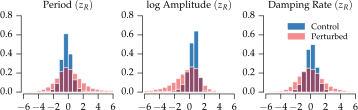
\includegraphics[]{figures/pdfs/fitted_parameters.pdf}
  \end{center}
  \caption{{\bfseries Figure Title.}
({\bfseries A}) Part A.
({\bfseries B}) Part B.}
\label{fig:fit_distributions}
\end{figure}


\begin{table}
  \begin{center}
    \begin{tabular}{lrrrrrr}\toprule
      {} & \multicolumn{2}{c}{$T$} & \multicolumn{2}{c}{$\ln A$} & \multicolumn{2}{c}{$d$} \\
      {}         & \multicolumn{1}{c}{C}         & \multicolumn{1}{c}{P}           & \multicolumn{1}{c}{C}         & \multicolumn{1}{c}{P}               & \multicolumn{1}{c}{C}         & \multicolumn{1}{c}{P}           \\\midrule
      $\mu$      & $-0.234$  & $0.187$  &  $0.443$  & $-0.343$  &  $0.043$  & $0.090$    \\
      $\sigma$   & $ 0.774$  & $1.820$  &  $0.778$  & $ 1.753$  &  $0.878$  & $1.688$    \\
      Skew & $ 0.153$  & $0.367$  & -$1.823$  & $-0.580$  & -$0.107$  & $0.371$    \\
      Kurt & $ 3.772$  & $0.591$  &  $8.329$  & $ 0.476$  &  $2.423$  & $0.373$    \\
      \bottomrule
    \end{tabular}
  \end{center}
  \caption{{\bfseries Fitted Parameters}}
  \label{tab:fit_distributions}
\end{table}


\begin{table}
  \begin{center}
    \begin{tabular}{rrrrr}
      \toprule
      {}       & $d$    & $\ln A$ & $T$    & $\theta$ \\\midrule
      $d$      & $1.000 $ & $0.285 $  & $-0.142$ & $-0.269$\\\
      $\ln A$  & $0.285 $ & $1.000 $  & $-0.022$ & $-0.112$\\
      $T$      & $-0.142$ & $-0.022$  & $1.000 $ & $-0.113$\\
      $\theta$ & $-0.269$ & $-0.112$  & $-0.113$ & $1.000 $\\
      \bottomrule
    \end{tabular}
  \end{center}
  \caption{{\bfseries Correlation matrix}}
  \label{tab:corr}
\end{table}


\begin{figure}[tbp]
  \begin{center}
    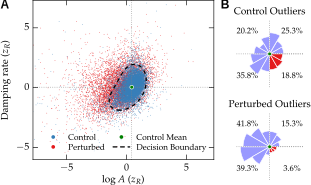
\includegraphics[]{figures/pdfs/outliers.pdf}
  \end{center}
  \caption{{\bfseries Figure Title.}
({\bfseries A}) Part A.
({\bfseries B}) Part B.}
\label{fig:outlier_dist}
\end{figure}




\section*{Conclusion}

\section*{Acknowledgments}
This work was supported by the National Institutes of Health/National Institute of General Medical Sciences under award number 1R01GM096873-01 and by the Institute for Collaborative Biotechnologies through grant W911NF-09-0001 from the U.S.\ Army Research Office.


\bibliographystyle{msb}
\bibliography{library.bib}

\beginsupplement

\begin{figure}[tbp]
  \begin{center}
    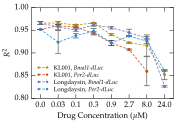
\includegraphics[]{figures/pdfs/small_molecule_r2.pdf}
  \end{center}
  \caption{{\bfseries Figure Title.}
({\bfseries A}) Part A.
({\bfseries B}) Part B.}
\label{fig:small_molecule_r2}
\end{figure}

\begin{figure}[tbp]
  \begin{center}
    \includegraphics[]{figures/pdfs/volume_calibration.pdf}
  \end{center}
  \caption{{\bfseries Figure Title.}
({\bfseries A}) Part A.
({\bfseries B}) Part B.}
\label{fig:vol_calibration}
\end{figure}

\begin{figure}[tbp]
  \begin{center}
    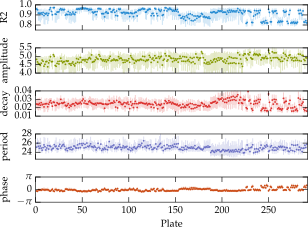
\includegraphics[]{figures/pdfs/zhang_plates.pdf}
  \end{center}
  \caption{{\bfseries figure title.}
({\bfseries a}) part a.
({\bfseries b}) part b.}
\label{fig:plate_variation}
\end{figure}

\begin{figure}[tbp]
  \begin{center}
    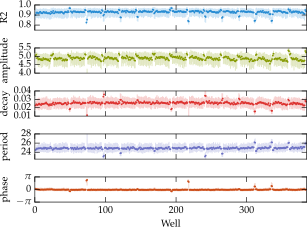
\includegraphics[]{figures/pdfs/zhang_wells.pdf}
  \end{center}
  \caption{{\bfseries figure title.}
({\bfseries a}) part a.
({\bfseries b}) part b.}
\label{fig:well_variation}
\end{figure}

\begin{table}
\begin{center}
\begin{tabular}{lclc}
\toprule
\textbf{Dep. Variable:}    &      Damping Rate       & \textbf{  R-squared:         } &$     0.169  $\\
\textbf{Model:}            &       OLS        & \textbf{  Adj. R-squared:    } &$     0.169  $\\
\textbf{Method:}           &  Least Squares   & \textbf{  F-statistic:       } &$     4782.  $\\
\textbf{Date:}             & Wed, 11 Feb 2015 & \textbf{  Prob (F-statistic):} &$     0.00   $\\
\textbf{Time:}             &     16:26:22     & \textbf{  Log-Likelihood:    } &$-1.7248e+05 $\\
\textbf{No. Observations:} &       94053      & \textbf{  AIC:               } &$ 3.450e+05  $\\
\textbf{Df Residuals:}     &       94048      & \textbf{  BIC:               } &$ 3.450e+05  $\\
\bottomrule
\end{tabular}
\begin{tabular}{lccccc}
                   & \textbf{coef} & \textbf{std err} & \textbf{t} & \textbf{P$>$$|$t$|$} & \textbf{[95.0\% Conf. Int.]}  \\
\midrule
\textbf{const}     &     $-0.0370$ &       $0.014$    &   $-2.572$ &        $0.010$       &       $-0.065,  -0.009$      \\
\textbf{amplitude} &     $ 0.2375$ &       $0.003$    &   $86.282$ &        $0.000$       &       $ 0.232,   0.243$      \\
\textbf{period}    &     $-0.1521$ &       $0.003$    &   $56.798$ &        $0.000$       &       $-0.157,  -0.147$      \\
\textbf{phase}     &     $-0.2354$ &       $0.003$    &   $85.598$ &        $0.000$       &       $-0.241,  -0.230$      \\
\textbf{type}      &     $ 0.3197$ &       $0.015$    &   $20.664$ &        $0.000$       &       $ 0.289,   0.350$      \\
\bottomrule
\end{tabular}
\begin{tabular}{lclc}
\textbf{Omnibus:}       &$9769.391$& \textbf{  Durbin-Watson:     } &$    1.876$ \\
\textbf{Prob(Omnibus):} &$  0.000 $& \textbf{  Jarque-Bera (JB):  } &$18459.719$ \\
\textbf{Skew:}          &$  0.697 $& \textbf{  Prob(JB):          } &$     0.00$ \\
\textbf{Kurtosis:}      &$  4.664 $& \textbf{  Cond. No.          } &$     8.34$ \\
\bottomrule
\end{tabular}
\end{center} 
\caption{OLS Regression Results}
\label{tab:ols_reg}
\end{table}


\end{document}

